\section{RP14 Unobtrusive JavaScript}
\label{sec:principle-rp14-unobtrusive-javascript}

Aktuelle Webapplikationen können grob in zwei Kategorien eingeteilt werden:

\begin{figure}[H]
	\begin{table}[H]
		\tablestyle
		\tablealtcolored
		\begin{tabularx}{\textwidth}{l l X}
			\tableheadcolor
				\tablehead Kategorie &
				\tablehead Beispiel &
				\tablehead Erläuterung
				\tabularnewline
			\tablebody
				Server-Rendering &
				\emph{GitHub} \cite{GitHub} &
				User Interface wird auf dem Server gerendert, JavaScript bringt lediglich dynamisch geladene Inhalte, Effekte oder zusätzliche ``optionale'' Features.
				\tabularnewline

				JavaScript Client &
				\emph{Google Drive} \cite{GoogleDrive} &
				User Interface wird komplett im Browser mittels JavaScript aufgebaut. Ohne JavaScript keine Funktionalität oder schlechtere User Experience.
				\tabularnewline
			\tableend
		\end{tabularx}
	\end{table}
	\caption{Kategorien aktueller Webapplikationen}
	\label{tab:current-webapplication-categories}
\end{figure}

Die Kategorie \emph{Server-Rendering} zeichnet sich durch eine hohe Kompatibilität mit allen möglichen Internetbrowsern aus. Durch die Generierung des HTML Markups losgelöst vom schlussendlichen Zielclient, liegt die ganze Verantwortung, vom beschaffen anzuzeigender Daten bis hin zum zusammenstellen des HTML \gls{DOM}'s komplett bei der Serverkomponente.

Zwar kommt auch bei diesem Typus oftmals JavaScript zur Anwendung, meist beschränkt sich dessen Anwendung aber auf die Ergänzung des bereits statisch geladenen Inhaltes. So lädt \emph{Mila} \cite{Mila} beim Seitenwechsel, sofern JavaScript aktiviert, neuen Inhalt über einen \gls{AJAX} Request. Nach Erhalt des vorgerenderten HTML Markups aus der Antwort ersetzt es entsprechende Inhalte im aktuell angezeigten HTML \gls{DOM} des Browsers.

Als Programmiersprache auf dem Applikationsserver kommt hier oft Java, PHP, Ruby o.Ä. zum Einsatz.

Beim puren \emph{JavaScript Client} liegt der Programmcode für das Rendern des User Interfaces mit all seinen Inhalten als JavaScript Quelltext vor. Nach erfolgreicher Übertragung zum Internetbrowser initiiert dieser die Erstellung der Applikationsoberfläche im HTML \gls{DOM} des Clients.

Sollen dynamische Informationen angezeigt werden, müssen diese über eine Serviceschnittstelle beim entsprechenden Anbieter angefragt werden (siehe bspw. Abschnitt \ref{sec:principle-rp1-rest} ``\nameref{sec:principle-rp1-rest}'').

Es ist zu erahnen, dass diese Art von Webapplikation ohne JavaScript-Unterstützung im Browser des Endbenutzers nicht ausgeführt werden kann. Ein Beispiel hierfür liefert der \emph{Google Drive} \cite{GoogleDrive} Webclient. Wie in Abbildung \ref{fig:googleDriveNoJs} ersichtlich verweigert dieser ohne aktiviertes JavaScript die Funktion und zeigt ein leeres Standardlayout mit einer entsprechenden Meldung an.

\begin{figure}[H]
	\centering
	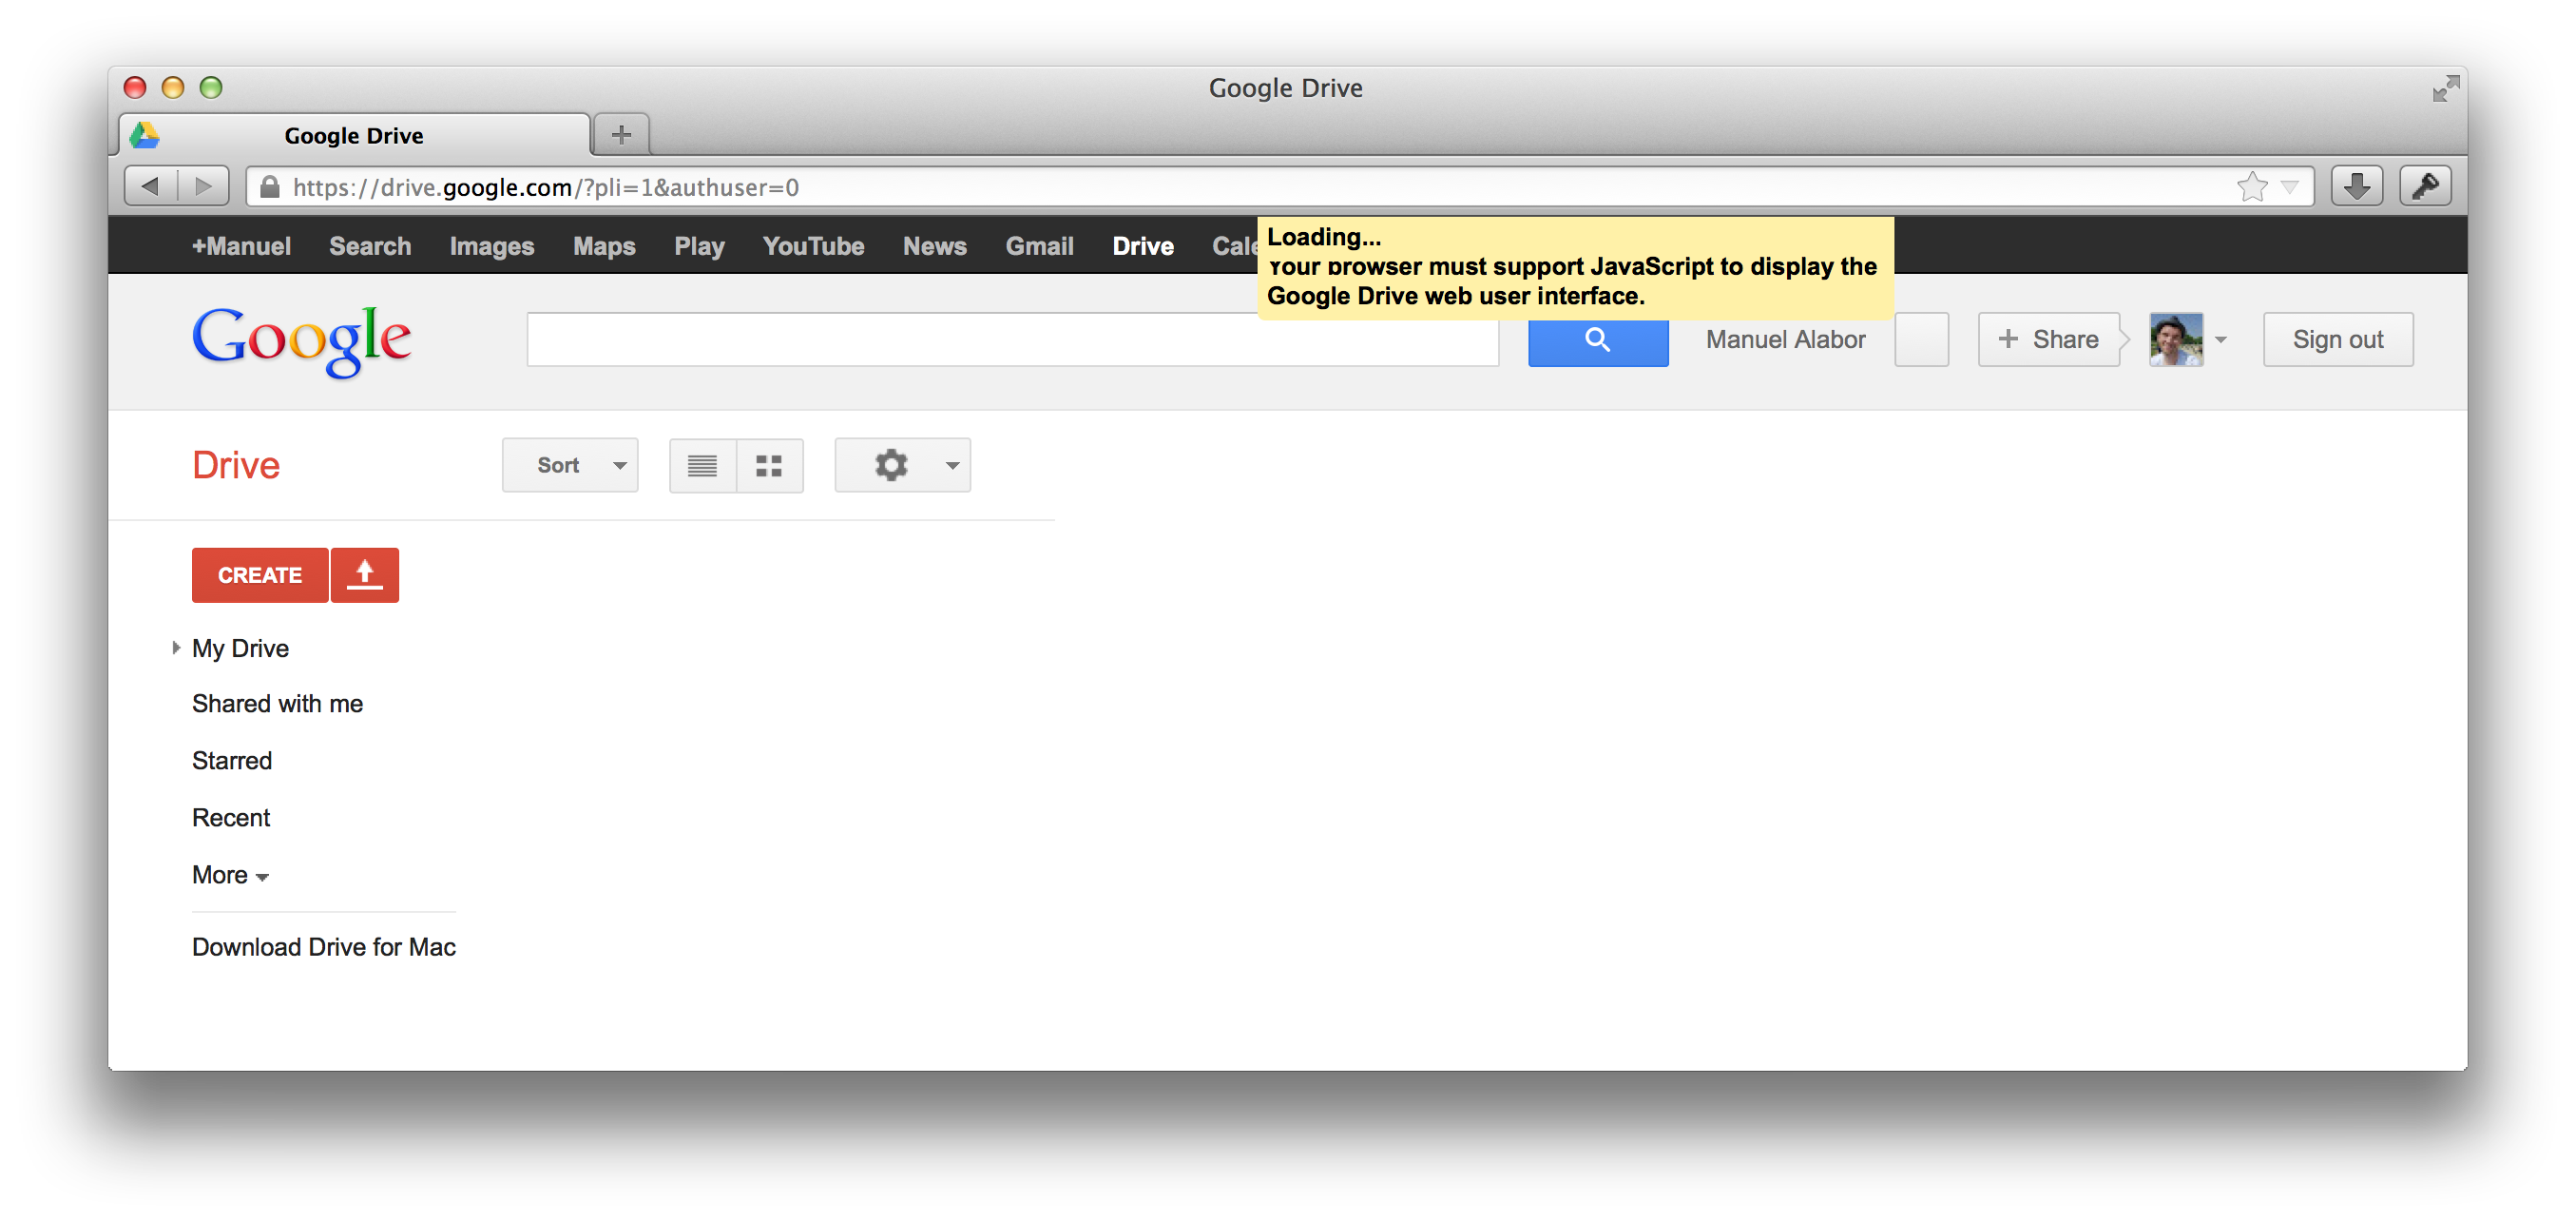
\includegraphics[width=12cm]{content/principle-demonstration/images/googledrive-nojs.png}
	\caption{\emph{Google Drive} in Firefox 21.0 mit deaktiviertem JavaScript}
	\label{fig:googleDriveNoJs}
\end{figure}



\subsection*{Geplante Umsetzung}


\subsection*{Konkrete Umsetzung}


\subsection*{Diskussion}
